\documentclass[12pt]{article}


\usepackage{amssymb}
\usepackage{amsmath}
\usepackage{fullpage}
\usepackage{epsfig}
\usepackage{epstopdf}
\everymath{\displaystyle}

\newif\ifans

\anstrue

\begin{document}

\begin{center}
\underline{\LARGE{Chapter 4.5 Practice Problems}}
\end{center}

\noindent EXPECTED SKILLS:

\begin{itemize}

\item Know how to use the techniques from Chapter 4.4 to solve optimization problems, i.e. given a system of related quantities, find values of the quantities that optimize one of them (e.g. minimize a cost, maximize a volume, etc)

\end{itemize}

\noindent PRACTICE PROBLEMS:

\medskip

\begin{enumerate}

\item A rectangle is to be inscribed with its base on the $x$-axis and its upper corners on the parabola $y=27-x^2$.  What are the dimensions of such a rectangle with the greatest possible area?

\ifans{\fbox{The dimensions of such a rectangle with the greatest area are 6 by 18.}} \fi

\item A rectangular plot of farmland is is bounded on one side by a straight river bank and on the other three sides by a single-strand electric fence.  If you are to use 3600 meters of wire to construct the fence, what is the largest area that you can enclose?  And, what are the dimensions of rectangular plot with the maximal area?

\ifans{\fbox{\parbox{1\linewidth}{The side parallel to the river should be 1800 meters long.  The remaining two sides of the fence should each be 900 meters long.  The maximal encolsed area is 1,620,000 square meters.}}} \fi

\item A fence must be built to enclose a rectangular area of 3000 square feet.  Fencing material costs \$5 per foot for the north and south sides.  And, it costs \$3 per foot for the other two sides.  Find the cost of the least expensive fence.

\ifans{\fbox{The least expensive fence costs \$$600\sqrt{2}$ which is approximately \$848.53.}} \fi

\item An open top box is to be constructed from a 7 inch by 15 inch piece of cardboard by cutting out a square of equal size from each of the four corners and then folding up the resulting sides.

\begin{enumerate}

\item What size square should be cut from each of the four corners in order to maximize the volume of the resulting box?

\ifans{\fbox{A square with a side length of 1.5 inches should be cut from each corner.}} \fi

\item What are the dimensions of the box with maximal volume?

\ifans{\fbox{1.5 inches by 4 inches by 12 inches}} \fi

\item What is the maximum volume for such a box?

\ifans{\fbox{72 cubic inches}} \fi

\end{enumerate}

\item What are the dimensions of the rectangle with the maximal area that can be inscribed in a circle of radius $5\sqrt{2}$?

\ifans{\fbox{10 by 10}} \fi

\item A rectangular tank with a square base, an open top, and a volume of 108 cubic yards is to be constructed of sheet metal.  Find the dimensions of the tank that has the minimal surface area.

\ifans{\fbox{6 yards by 6 yards by 3 yards}} \fi

\item You would like to frame a 27 square inch rectangular print of the Drexel Dragon (as in the diagram below).  The top and bottom borders of the frame are 2 inches and 4 inches, respectively.  And, the side borders of the frame are each 1 inch.

\begin{center}
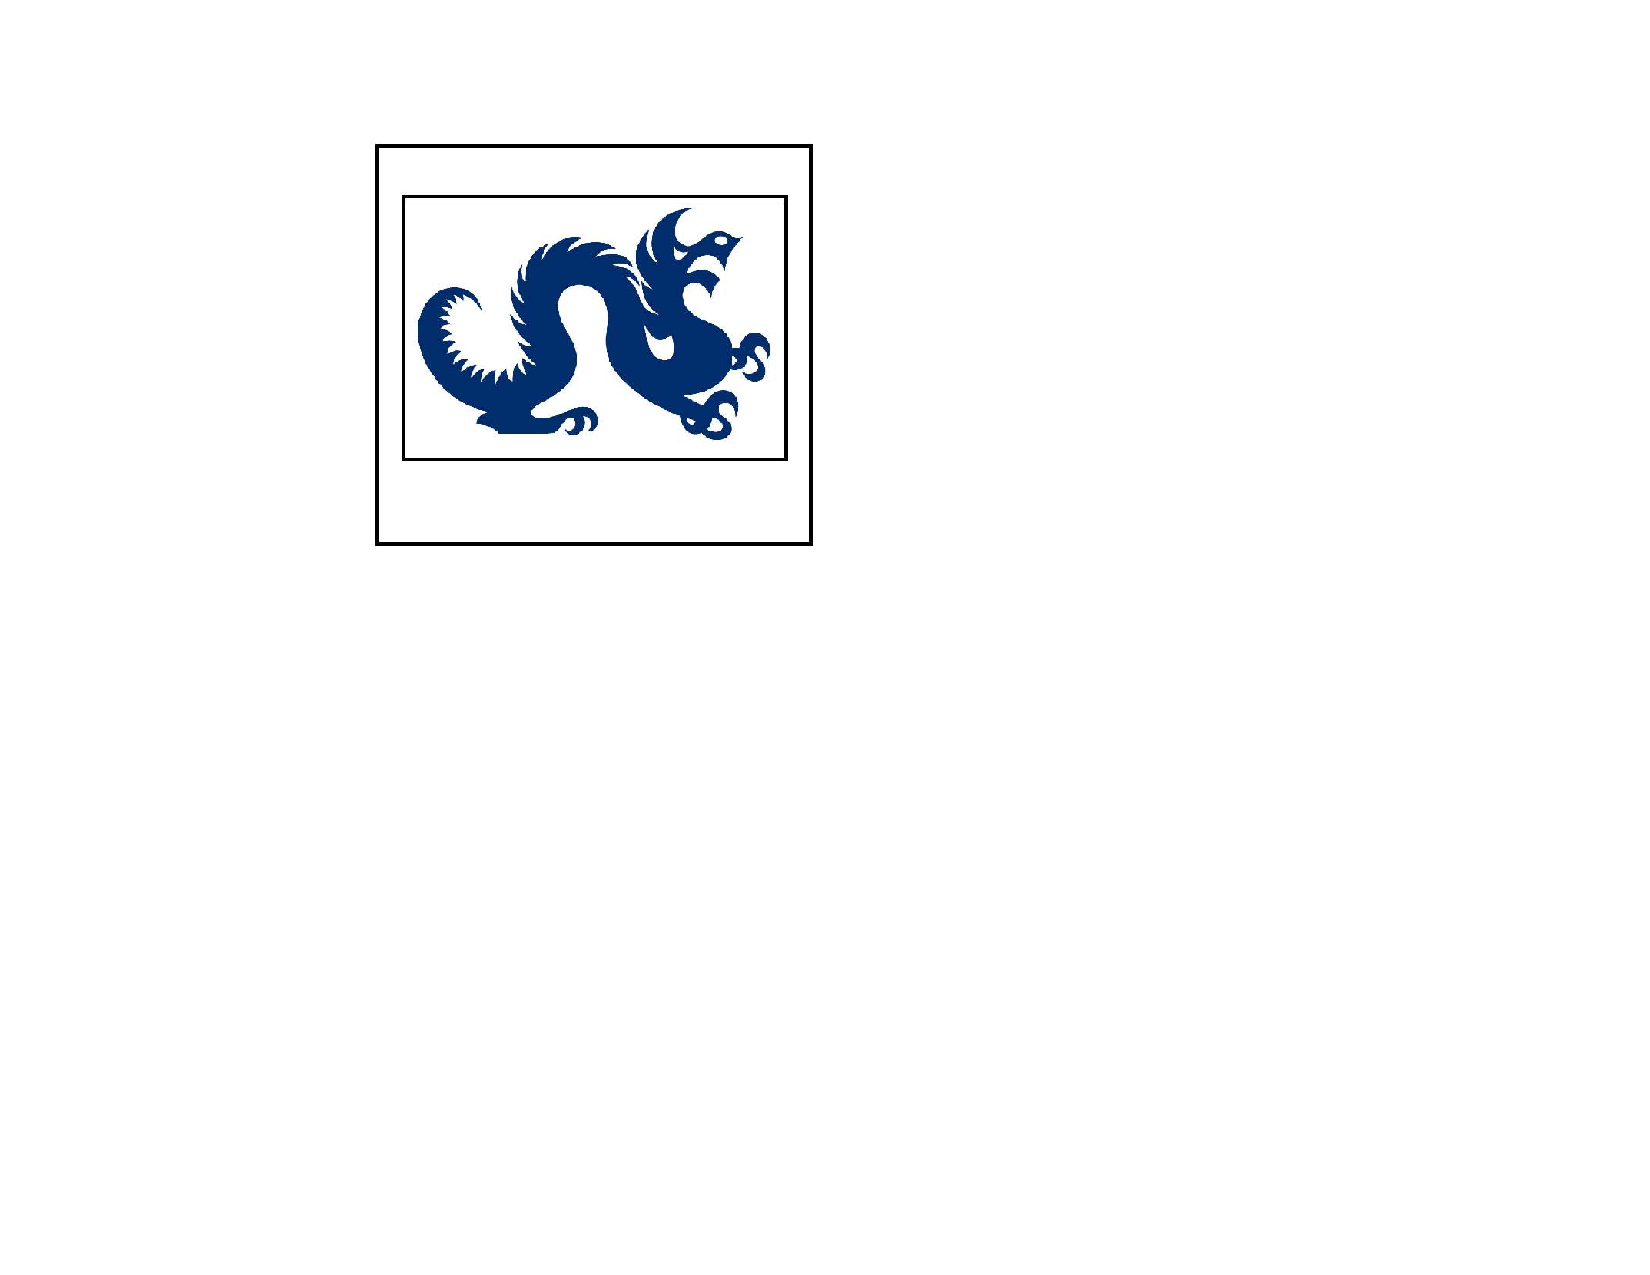
\includegraphics[scale=0.7]{mario.pdf}
\end{center}

What are the dimensions of the print which, when framed, cover the minimal amount of wall space?

\ifans{\fbox{The print should be 3 inches by 9 inches}} \fi

\item A soup manufacturer sells cans of soup with a fixed volume of $V$.  Their soup cans are always in the shape of a right circular cylinder with a radius of $r$ and a height of $h$.  Find the dimensions of the soup can which uses the least amount of materials.

\ifans{\fbox{$r=\sqrt[3]{\frac{V}{2\pi}}$ and $h=\sqrt[3]{\frac{4V}{\pi}}$}} \fi

\item Find the radius and height of the right circular cylinder of largest volume that can be inscribed in a right circular cone which has a base radius of 6 inches and a height of 10 inches.  What is the maximal volume?  (HINT: Use similar triangles.)
\begin{center}
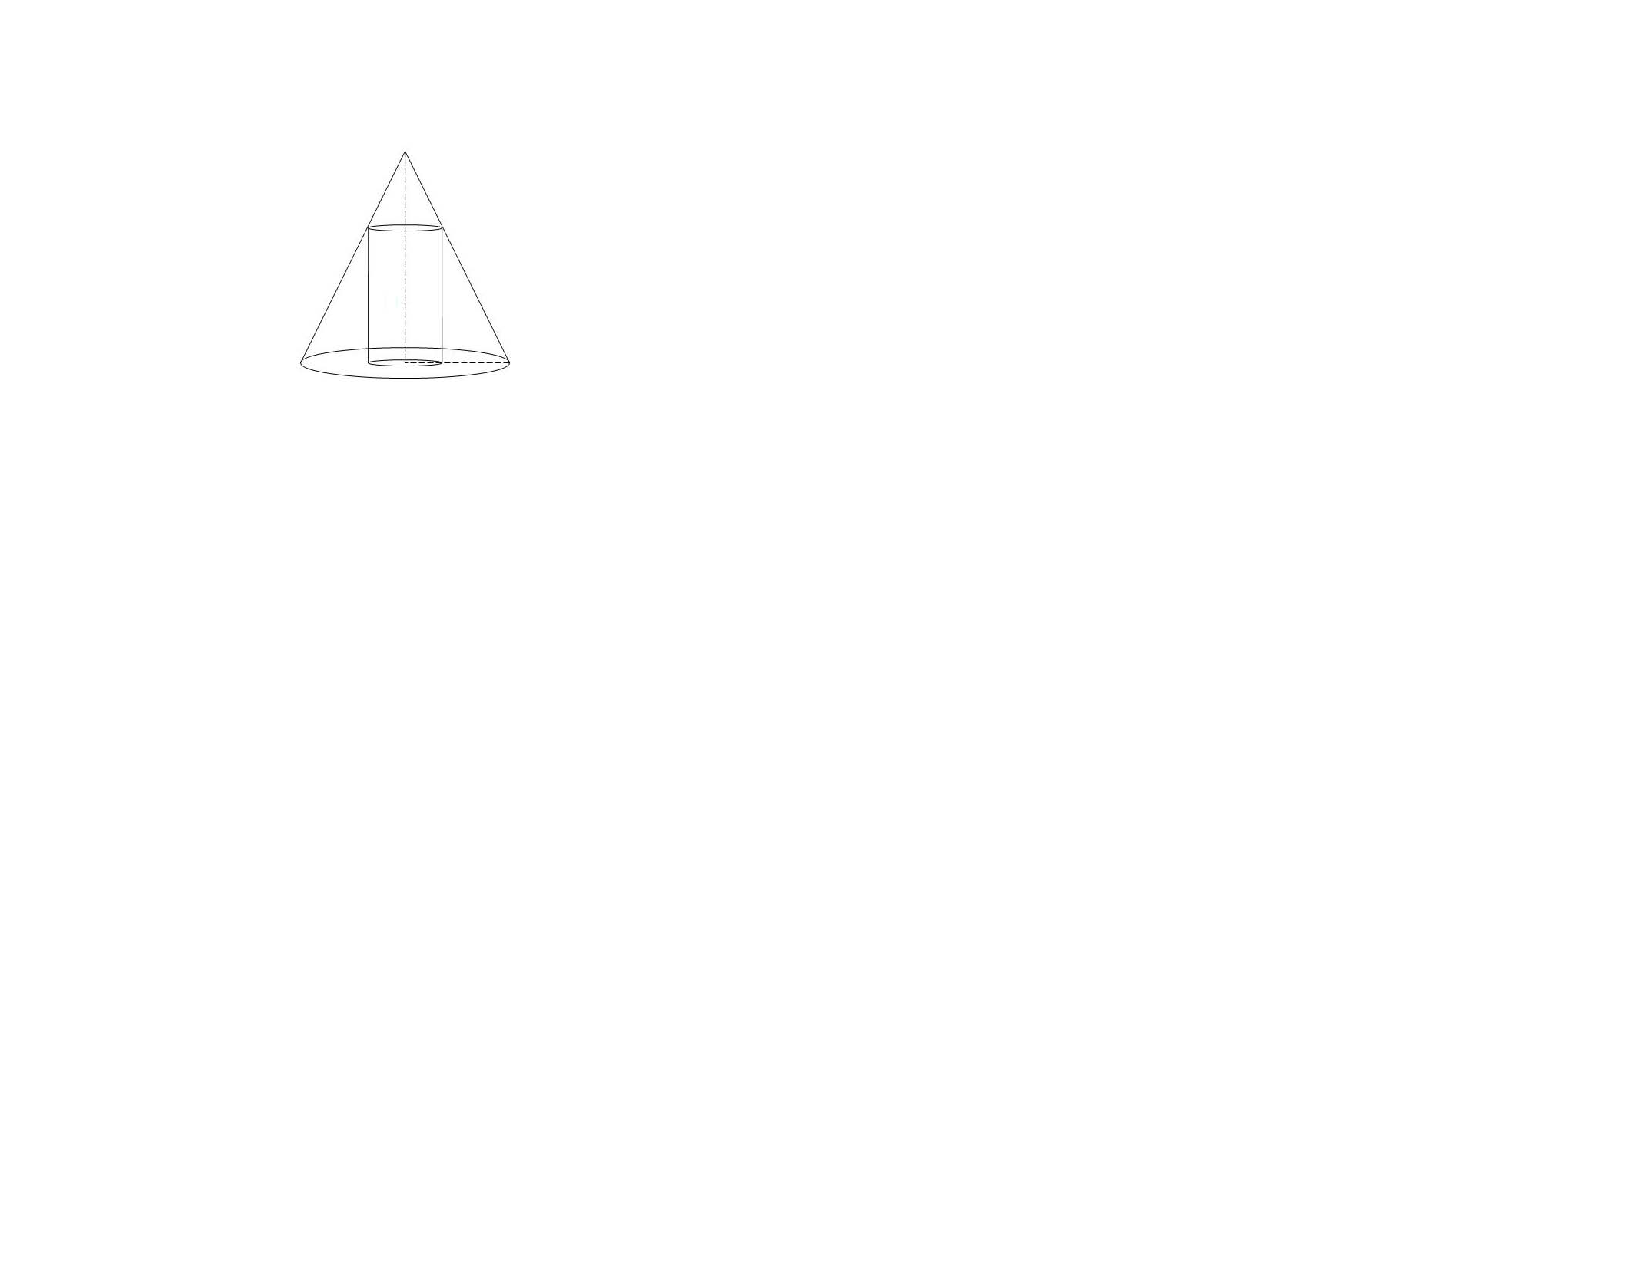
\includegraphics[scale=1]{cone.pdf}
\end{center}

\ifans{\fbox{$r=4$ inches, $h=\frac{10}{3}$ inches, and $V=\frac{160\pi}{3}$ cubic inches.}} \fi

\item A 24 inch long wire can be bent into the shape of either an equilateral triangle or a square.  Or, it can be cut into two pieces (not necessarily of equal length) to make both an equilateral triangle and a square.  How much wire should be used for the equilateral triangle if the total area enclosed by the shapes is to be

\begin{enumerate}

\item maximized?

\ifans{\fbox{0 inches; i.e., all of the wire should be used to make the square.}} \fi

\item minimized?

\ifans{\fbox{$\frac{216}{4\sqrt{3}+9}\approx13.56$ inches}} \fi

\end{enumerate}

\item Consider the curve $y=x^2$ for $0\leq x \leq 2$ and the point $P(3,0)$.

\begin{enumerate}

\item Find the point on the curve which is closest to $P$.

\ifans{\fbox{$(1,1)$ which is a distance of $\sqrt{5}$ from $P$.}} \fi

\item Find the point on the curve which is farthest from to $P$.

\ifans{\fbox{$(2,4)$ which is a distance of $\sqrt{17}$ from $P$}} \fi

\end{enumerate}

\end{enumerate}

\end{document}